\chapter{Internal Test}

\section*{Purpose}

The purpose was to test the system used in the expert review, including hardware load and frame times. This was done to determine whether potential issues could be attributed to physical limitations. Since the review and system test were both performed over LAN, no latency testing was performed.

\section*{Method}

The test was performed at Aalborg University's Audio-Visual Arena using the computers described in \autoref{tab:specs}. 

\begin{table}[H]
\centering
\begin{tabularx}{0.75\textwidth}{X X X}
\toprule
                     & \textit{Computer A} & \textit{Computer B} \\ \midrule \rowcolor{lightGrey}
\textbf{CPU}         & Intel Core i7-4770  & Intel Core i7-6700  \\

\textbf{GPU}         & Nvidia GTX 980      & Nvidia GTX 980    \\  \rowcolor{lightGrey}

\textbf{RAM} 		 & 16GB                & 16GB                 \\ \toprule
\end{tabularx}
\caption{Specifications of the computers used}
\label{tab:specs}
\end{table}

Two players and two observers were present. The players moved around in an introduction scene and in the final scene used in the system review. The observers recorded data using MSI Afterburner and Fraps to measure CPU and GPU load as well as framerate.

\section*{Results}
The results from the hardware monitoring are shown below. The range indicates roughly 10 minutes of play. The top graph shows GPU usage, the bottom shows CPU usage.

\begin{figure}[H]
\centering
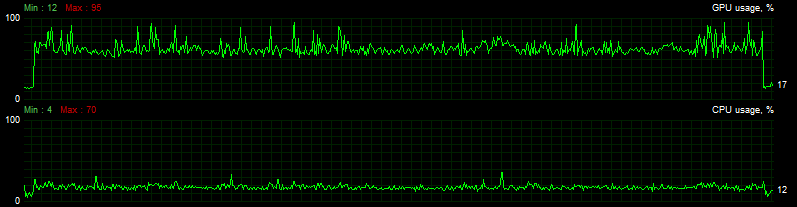
\includegraphics[width=0.95\textwidth]{InternalTest/B_usage.PNG}
\caption{Hardware usage of Computer A}
\end{figure}

\begin{figure}[H]
\centering
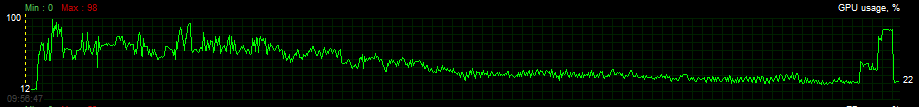
\includegraphics[width=0.95\textwidth]{InternalTest/C_gpu.PNG}
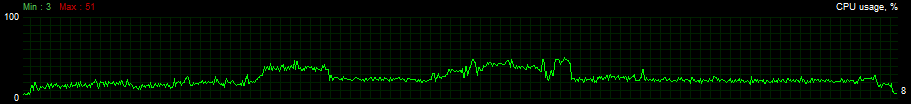
\includegraphics[width=0.95\textwidth]{InternalTest/C_cpu.PNG}
\caption{Hardware usage of Computer B}
\end{figure}

The results from recording framerate are shown below. 

\begin{figure}[H]
\centering
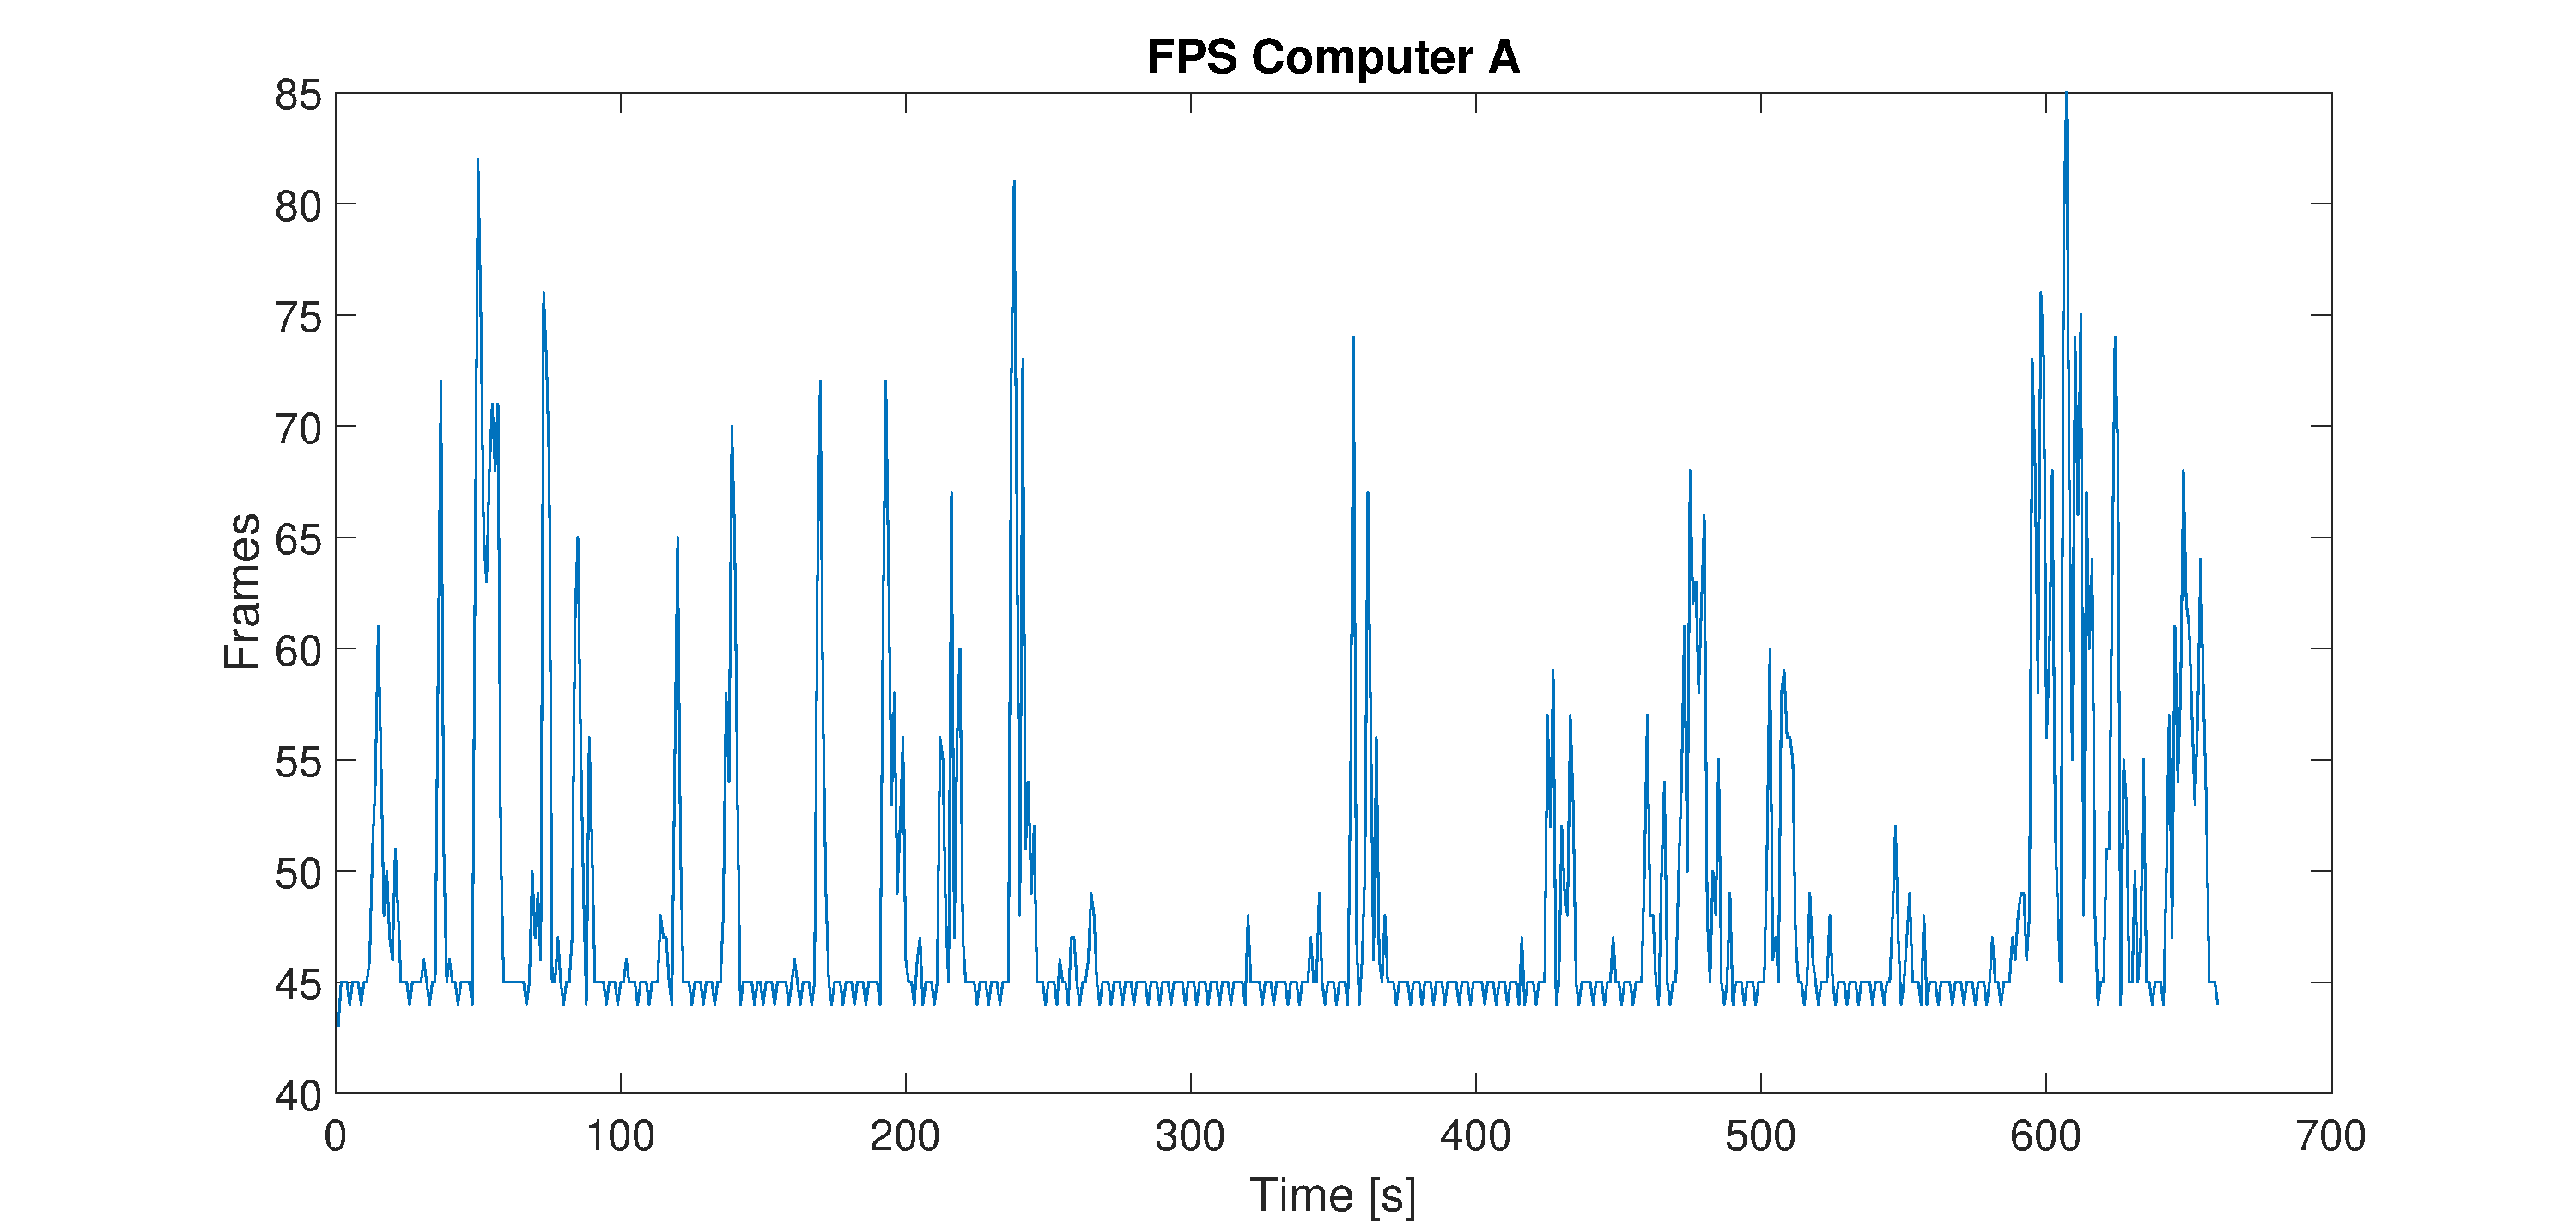
\includegraphics[width=0.95\textwidth]{InternalTest/A_fps.pdf}
\caption{Results from recording framerate in Computer A. Y-axis: Framecount, X-axis: Time in seconds}
\end{figure}

\begin{figure}[H]
\centering
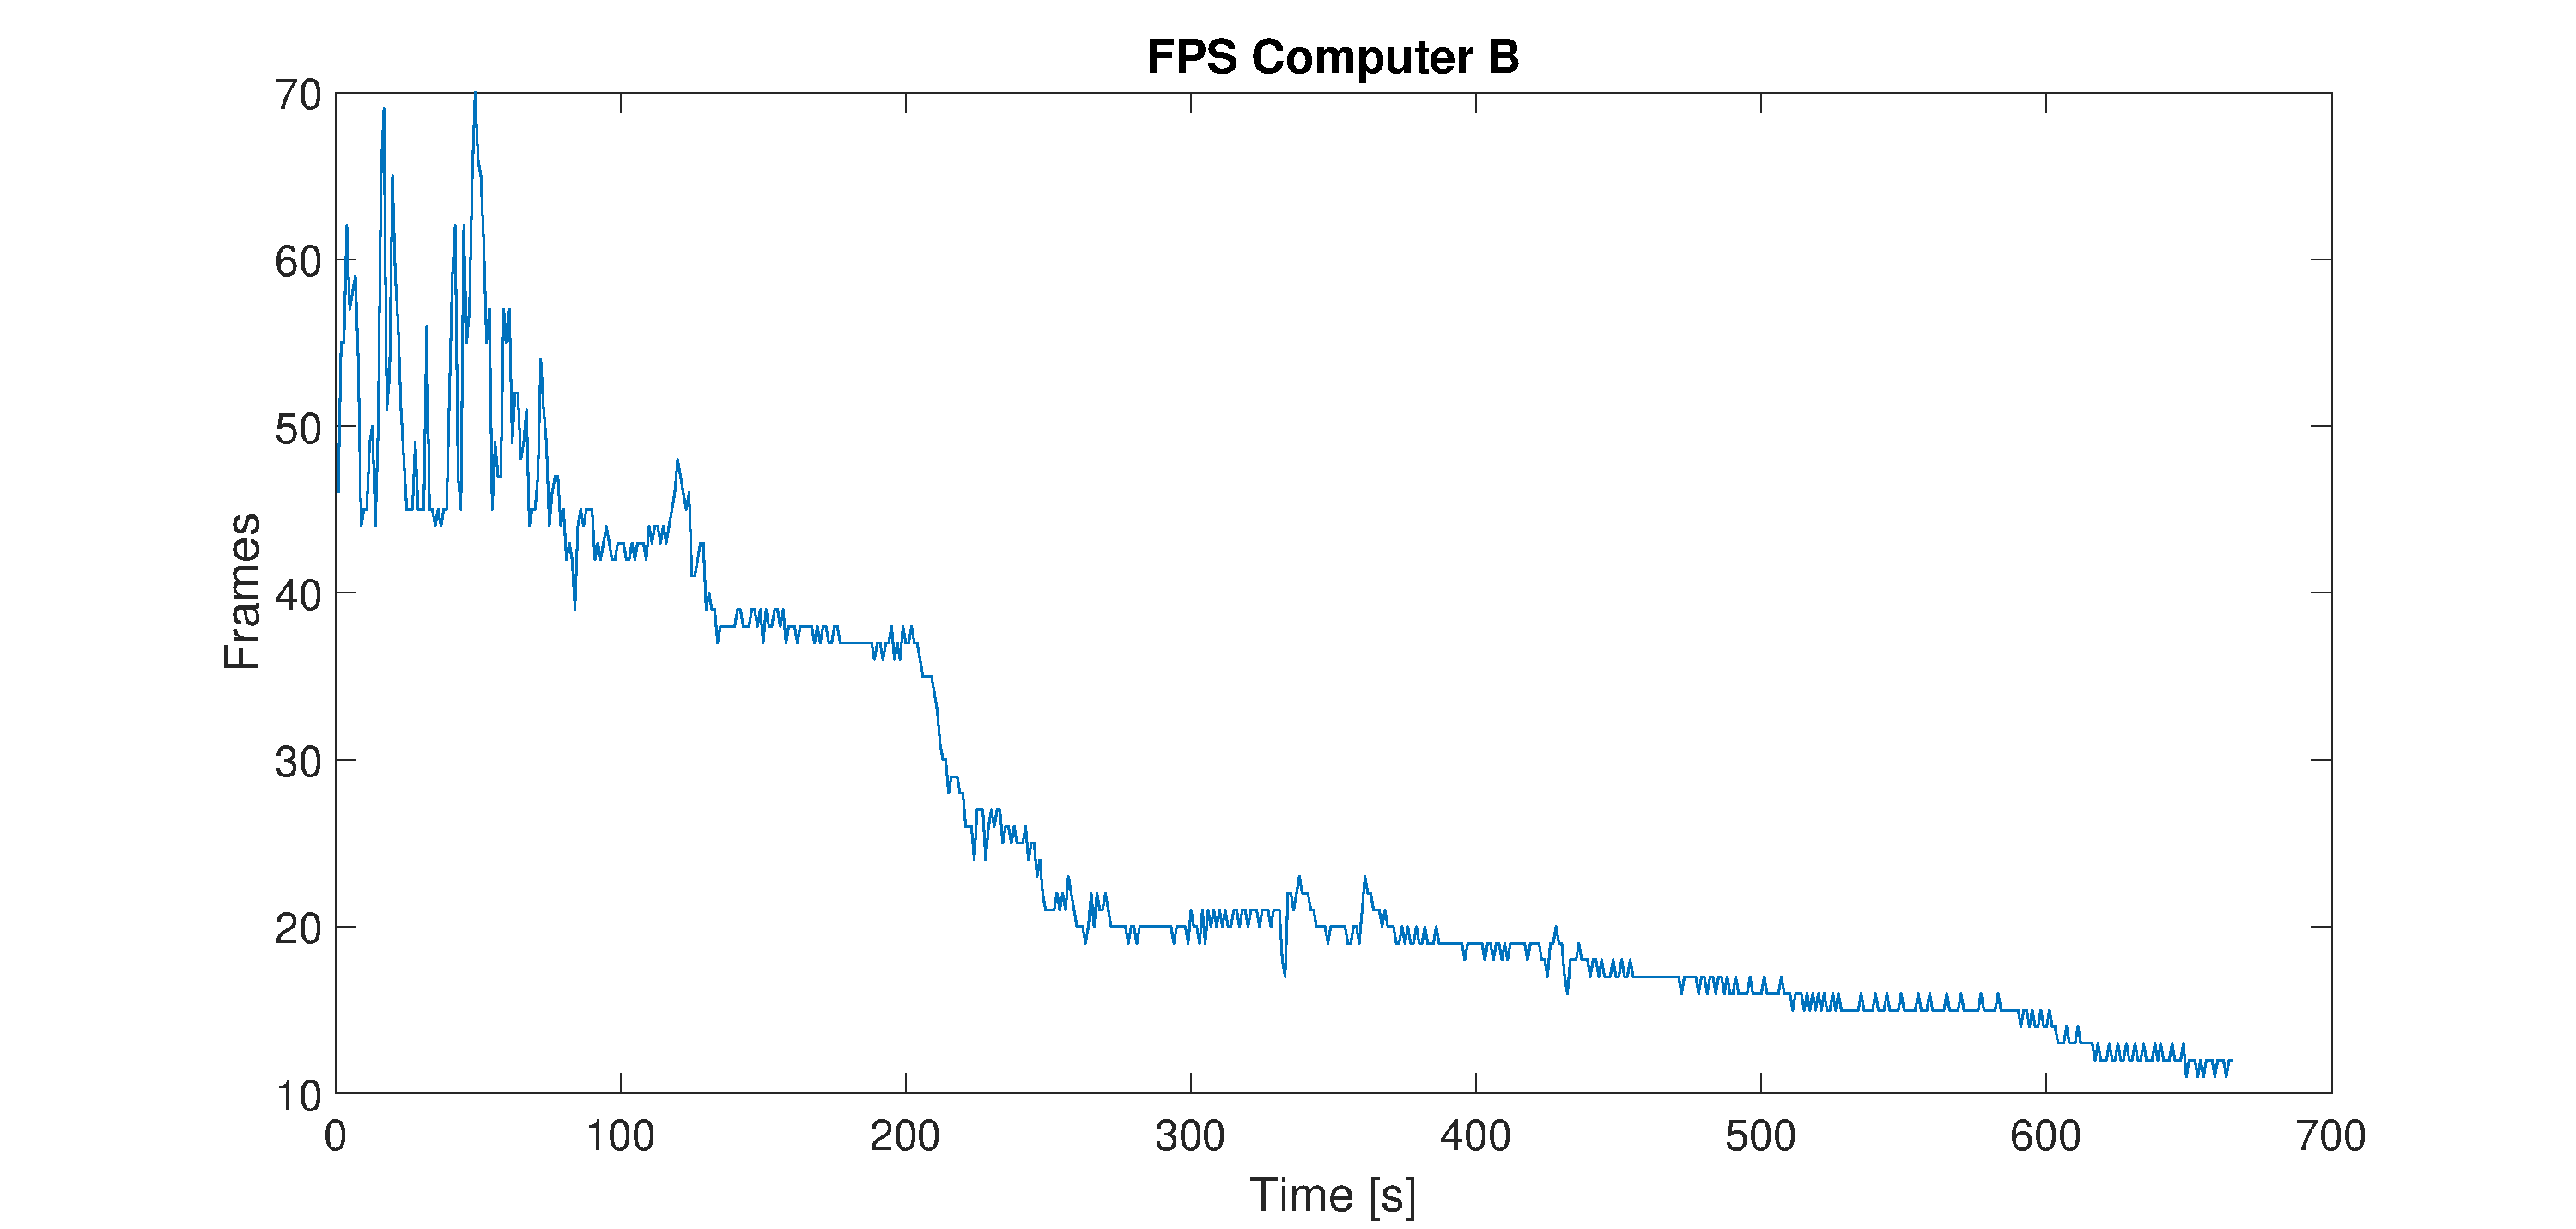
\includegraphics[width=0.95\textwidth]{InternalTest/B_fps.pdf}
\caption{Results from recording framerate in Computer B. Y-axis: Framecount, X-axis: Time in seconds}
\end{figure}


\section*{Conclusion}
The framerate results show a line at 45 frames per second, however monitoring in the same scene before beginning the recording showed a steady 90 frames per second. We hypothesize that the recording software is at fault, and cannot accurately record framerate in virtual reality applications. This was, however, the only possible solution since no native software that can log it was found. 

The results show a steady decline in framerate for the client computer. This was confirmed in several tests to be the case for any computer used as client, but does not seem to be caused by overheating. The client's GPU usage steadily drops while CPU usage seems to jump. This may be the fault of the Proteus multiplayer template for Unreal Engine, and the issue could be writing to a file or otherwise adding data to an array that must be processed at each frame. The issue can be fixed by starting the scene using "25 minutes play time" instead of 10 minutes.
